\section{Electronics} \index{Electronics}

\begin{multicols}{2}


\section*{Diodes} \index{Diodes}


\subsection{Forward and Reverse Biased Diodes}

\begin{center}
%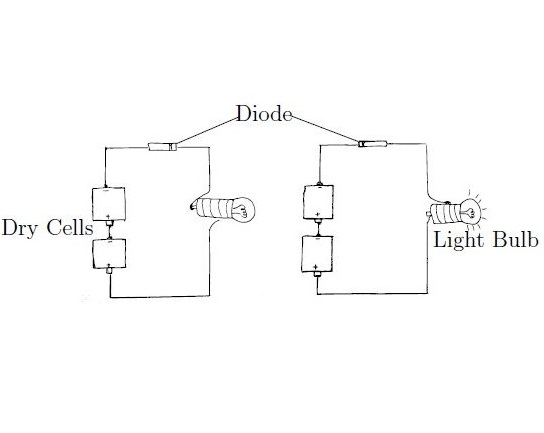
\includegraphics[width=0.6\textwidth]{./img/diodes.jpg}
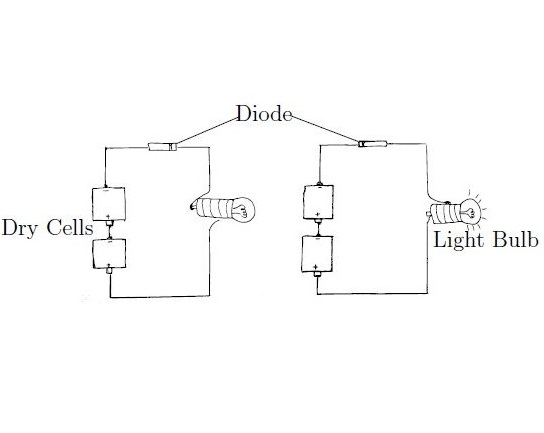
\includegraphics[width=0.5\textwidth]{./img/diodes.jpg}
\end{center}

\begin{description*}
%\item[Subtopic:]{}
\item[Materials:]{Diode, dry cell, bulb, connecting wires, nail, heat source or soldering iron}
\item[Setup:]{Remove a diode from a broken raido using a soldering iron or hot nail.}
\item[Procedure:]{Join the bulb in series with the P-N junction (diode). Connect the P-terminal of the junction to the positive terminal of the dry cell and the N-terminal of the junction to the negative terminal of the dry cell. Then reverse the terminals of the dry cell and observe any changes in the circuit.}
%\item[Hazards:]{}
%\item[Questions:]{}
\item[Observations:]{The bulb lights in the first arrangement, indicating that current is flowing. If the terminals are reversed, the bulb will not light, indicating that no current is flowing.}
\item[Theory:]{The P-N junction allows current to flow only in one direction; current can flow from the P-terminal to the N-terminal, but not the other way. Current always flows from a positive terminal to a negative terminal.}
\item[Applications:]{Radios, phone chargers, etc.}
\item[Notes:]{A diode has two colours: white and black. The black side is the P-terminal and the white band is the N-terminal. Current will only flow from the black side to the white side.}
\end{description*}

\vfill
\columnbreak

\subsection{Full-Wave Rectifier}

\begin{center}
%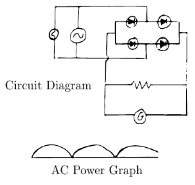
\includegraphics[width=0.7\textwidth]{./img/full-wave-rectifier-2.png}
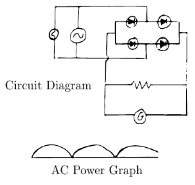
\includegraphics[width=0.5\textwidth]{./img/full-wave-rectifier-2.png}
\end{center}

\begin{description*}
%\item[Subtopic:]{}
\item[Materials:]{Low voltage AC power source (see \nameref{sub:inverter}), connecting wires, 4 diodes, bulb, resistor, galvanometer, optional super glue}
\item[Hazards:]{Do not use the power from outlets in a house or school.  These outlets put out a high voltage (220 V) which can kill you.  Instead use a laboratory power supply or use D-cell batteries with an inverter as described above.}
\item[Setup:]{Connect two diodes in series with connecting wire by using super glue or any other means. Repeat for another pair of diodes. Connect these pairs in parallel so that current can flow through either pair but only in one direction. Connect also a resistor and galvanometer in parallel across the pairs of diodes. Attach the AC power source to the middle of each diode pair using connecting wires. Attach a bulb in parallel across the AC source.}
\item[Procedure:]{Connect the AC source directly to the galvanometer and observe the behaviour of the galvanometer. Connect the AC source to the full-wave rectifier and observe the relation of the galvanometer in relation to the bulb.}
%\item[Questions:]{}
\item[Observations:]{When the AC source is connected directly to the galvanometer, the galvanometer needle will jump one direction and then the other, showing the changing direction of current through the circuit.  However, when the galvanometer is powered through the full-wave rectifier, it can be seen that the galvanometer only indicates one direction (positive or negative) and jumps quickly between zero and its maximum value.}
\item[Theory:]{If observed closely with an AC source of low frequency, it can be seen that the bulb and galvanometer flicker at exactly the same rate.  This is because the full-wave rectifier creates DC current which increases and decreases (but only in one direction) at the same frequency that the AC current is changing direction.  As the bulb is following the AC current at a certain frequency, the galvanometer is being driven by the DC current at the same frequency of increasing and decreasing.}
%\item[Applications:]{}
\item[Notes:]{This activity is normally done with an oscilloscope, which clearly shows the waveform of the AC current and rectified current.  However, the effect of the full-wave rectifier can be seen clearly if you are using the correct components.

First, the full-wave rectification can be compared to the half-wave rectification.  If you connect the AC source to both a half-wave rectifier and a full-wave rectifier, each with a galvanometer, it can be seen that the full-wave rectifier causes the galvanometer to move at twice the speed of the half-wave rectifier.

Also, when a bulb is attached in parallel across the AC source while the galvanometer reads the current through the full-wave rectifier, it can be seen that the bulb and galvanometer flicker at the same rate, proving that the entire AC wave is being converted directly to DC rather than only half of the wave.}
\end{description*}

\subsection{Half-Wave Rectifier}

\begin{center}
%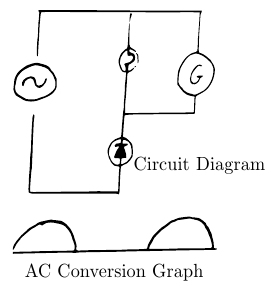
\includegraphics[width=0.7\textwidth]{./img/half-wave-rectifier-2.png}
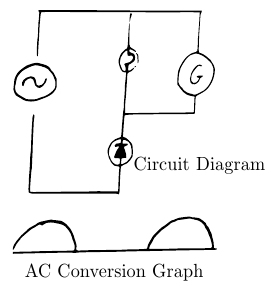
\includegraphics[width=0.5\textwidth]{./img/half-wave-rectifier-2.png}
\end{center}

\begin{description*}
%\item[Subtopic:]{}
\item[Materials:]{Low power AC power source (see \nameref{sub:inverter}), diode, bulb, galvanometer, connecting wires}
\item[Hazards:]{Do not use the power from outlets in a house or school.  These outlets put out a high voltage (220 V) which can kill you.  Instead use a laboratory power supply or use D-cell batteries with an inverter as described above.}
\item[Setup:]{Connect the P-side of a diode (the black colour indicates P-type) to one of the connecting wires from the power source. Connect one of the terminals of the bulb to the N-side of the diode (a white band indicates N-type). Connect the other terminal of the bulb to the remaining connecting wire of the power source. You should now have a power source, diode and bulb all in series. Connect the galvanometer in parallel with the bulb.}
\item[Procedure:]{Turn on the power and watch the behavior of the galvanometer.}
%\item[Questions:]{}
\item[Observations:]{When AC power is connected to a galvanometer, it is seen that the current is changing direction quickly, causing the needle to jump back and forth.  When the AC is passed through a half-wave rectifier, however, the current is only in one direction (positive or negative) and jumps between zero and the maximum value at half the speed that it did with AC current.}
\item[Theory:]{This is because the AC current is being cut in half through the rectifier and is allowed to move in only one direction.  If using a bulb, it will be seen that the bulb flickers quickly with AC current, but only half as quickly with half-wave rectified current.}
%\item[Applications:]{}
\item[Notes:]{This activity is normally done with an oscilloscope, which shows the wave pattern of the AC current (it is a sine wave).  If seen on the oscilloscope, the AC appears as a full sine wave, while the half-wave rectified current appears as only the positive or negative part of the sine wave (it looks like hills separated by long spaces).

A half-wave rectifier, rather than converting AC directly to DC, simply removes all current in one direction and allows all current in the other direction.  In this way, the product is direct current, but only half of what was produced by the AC power source.}
\end{description*}

%==================================================================================================%


\end{multicols}

\pagebreak